\section{User Interaction}\label{sec:interaction}
After initializing the flat mesh, we need to refine the model to final state through the shape constrain proposed and the information acquired from user interaction. The system provides a set of operations to assist users construct the optimized model, such as selecting points that need to be merged together. Moreover, the system can automatically detect the points that need to be located in one place and provide suggestions to allow users click the right option.

Figure~\ref{fig:interface} illustrates two operations that the system provides, the first one is selecting points need to be merged by users and the second is select the right option from results by auto-detection.   

\begin{figure}
	\centering
	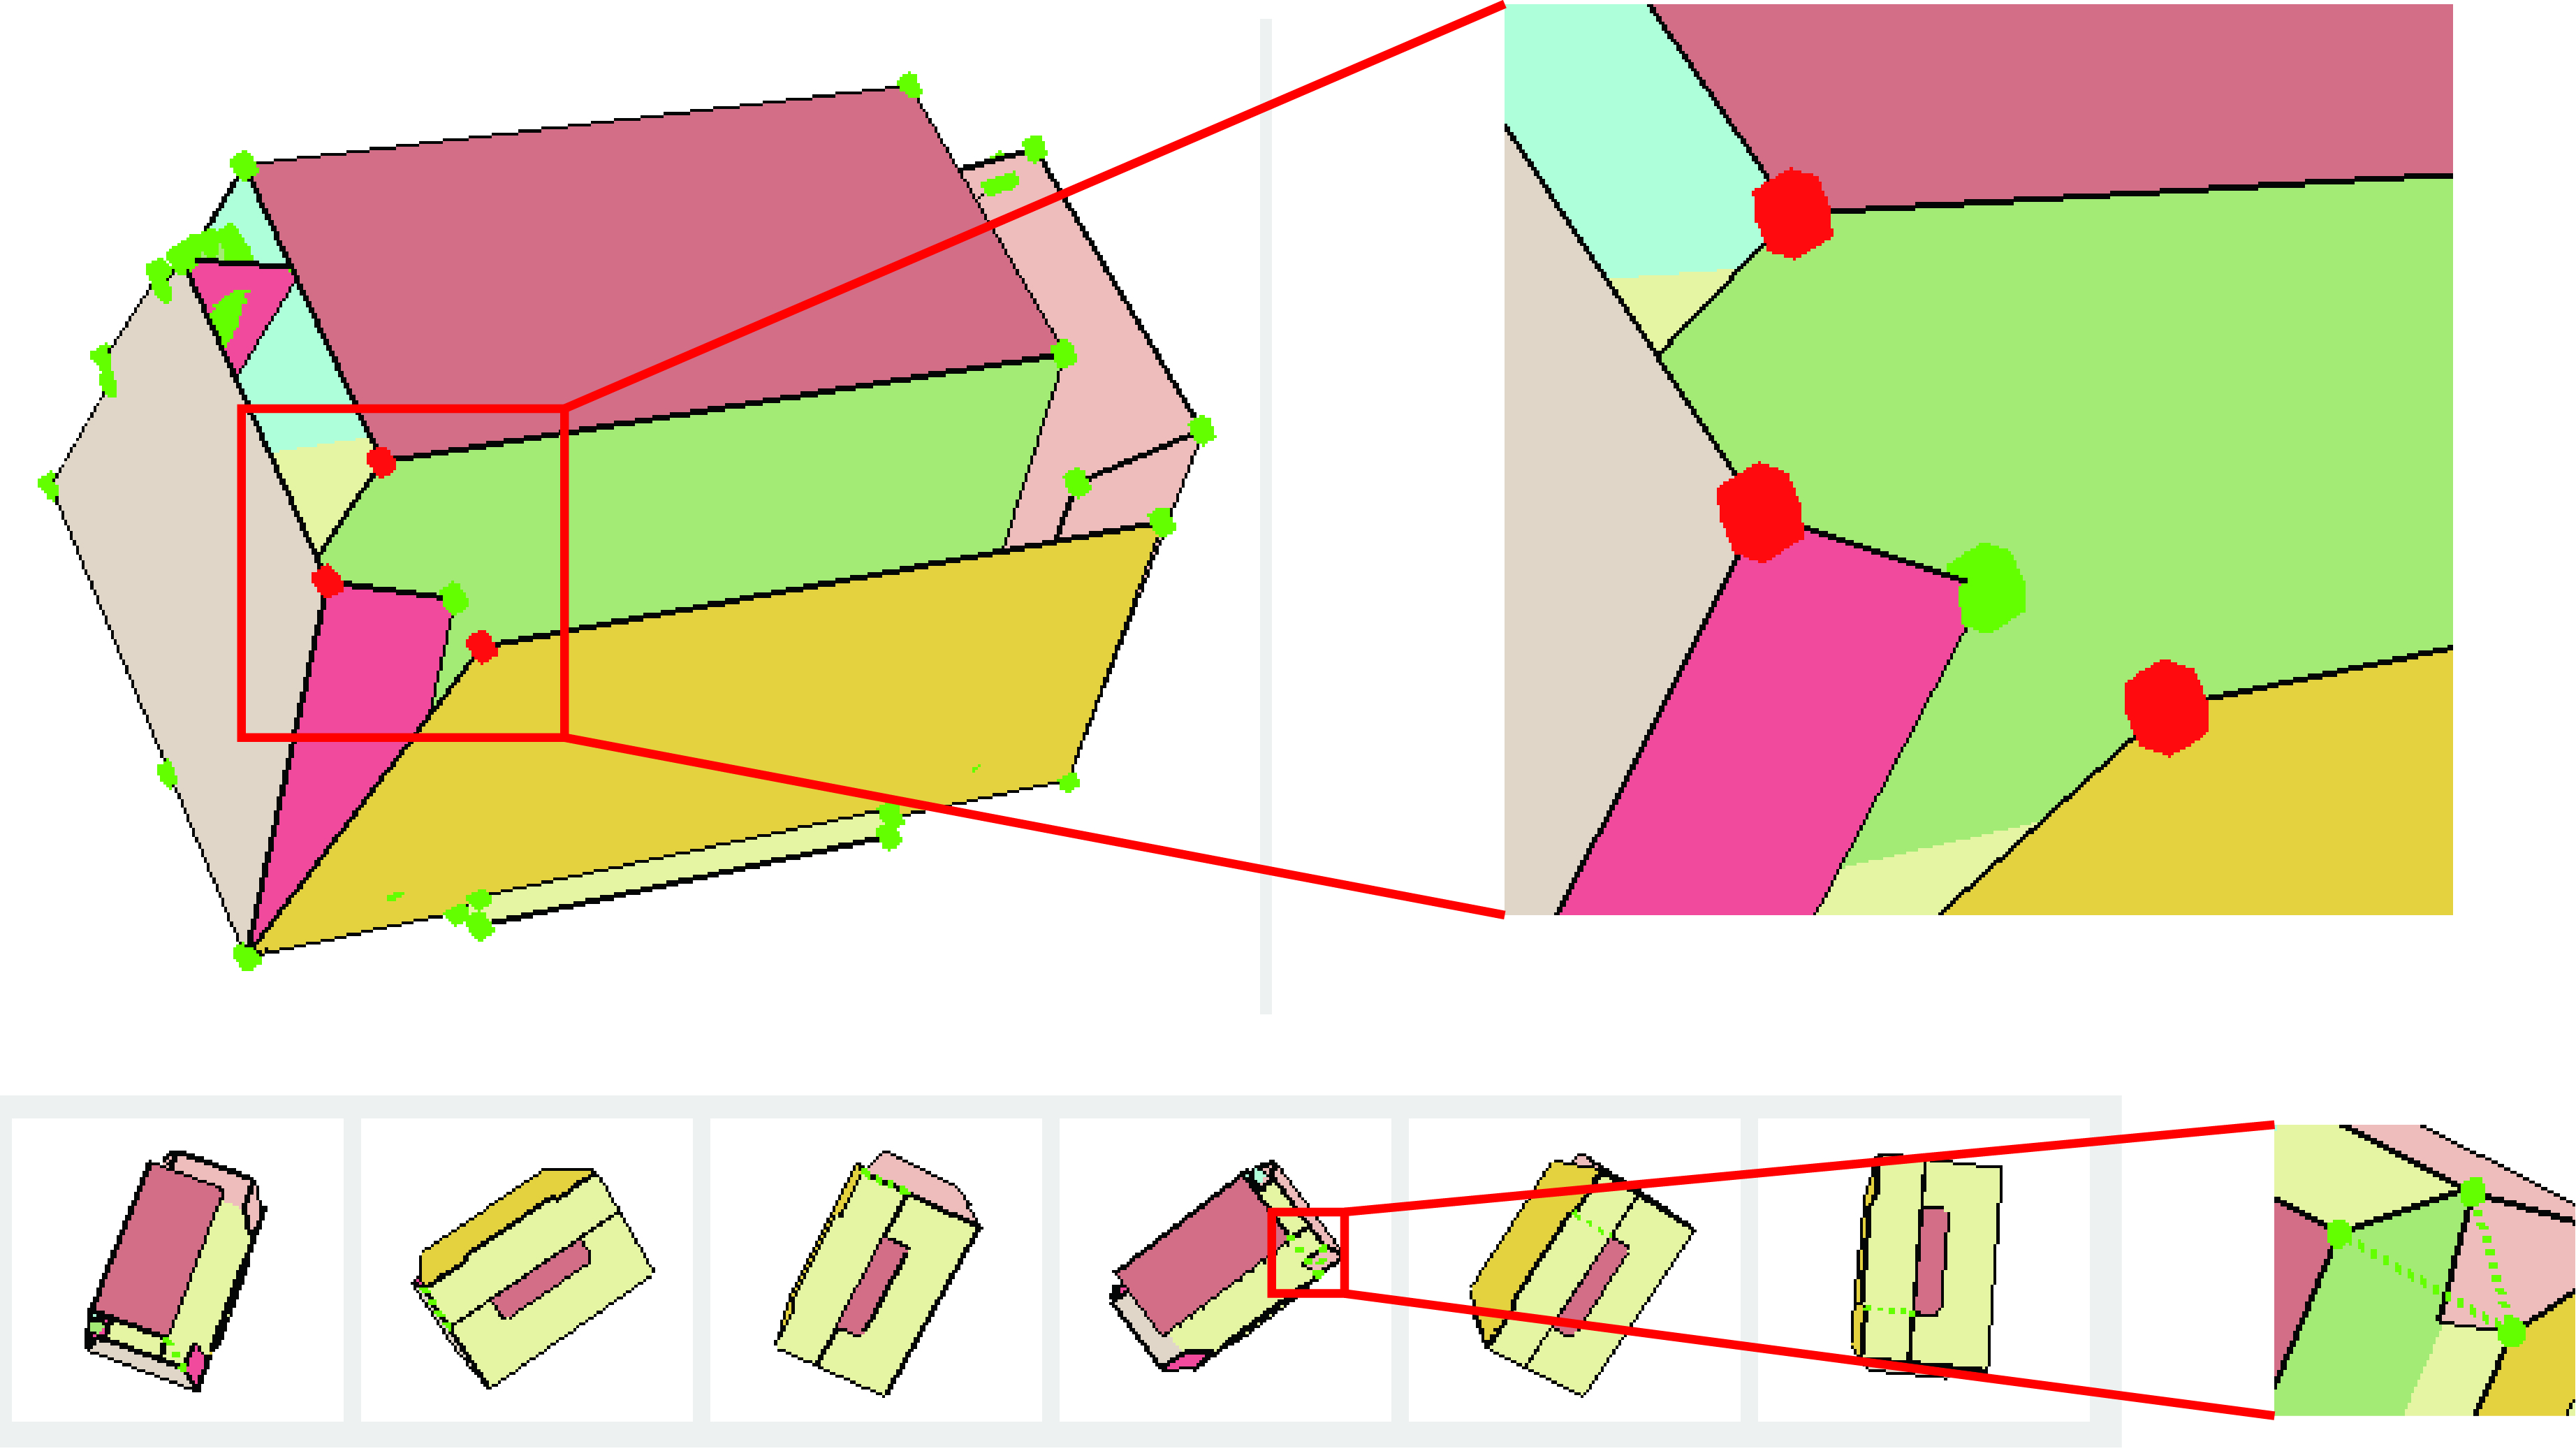
\includegraphics[width=0.9\textwidth]{images/UIdetail.jpg}
	\caption{two operations that the system provides}
	\label{fig:interface}
\end{figure}


\cxj{Explain when modify the 3D model, how to change the 2D layout. }